
\documentclass[10pt, letterpaper]{article}
%\usepackage{bookmark}
\usepackage[a4paper,margin=2cm]{geometry}
\usepackage[]{graphicx}
\usepackage{mathtools}
\usepackage{bm}
\usepackage[strings]{underscore}
\usepackage{apacite}
\setlength{\parindent}{0pt}
\graphicspath{ {./Images} }
\usepackage{wrapfig}
\usepackage[autostyle, english = american]{csquotes}
\usepackage[toc,page]{appendix}
\usepackage{amssymb}



\MakeOuterQuote{"}
\begin{document}
\begin{titlepage}
	\title{SOH-Coast-TOA: Modelling a roller coaster using trigonometric, cubic, and exponential functions}
	
	\author{Noah Alexiou}


	\date{March 2025}
	
	\maketitle
	\centering
	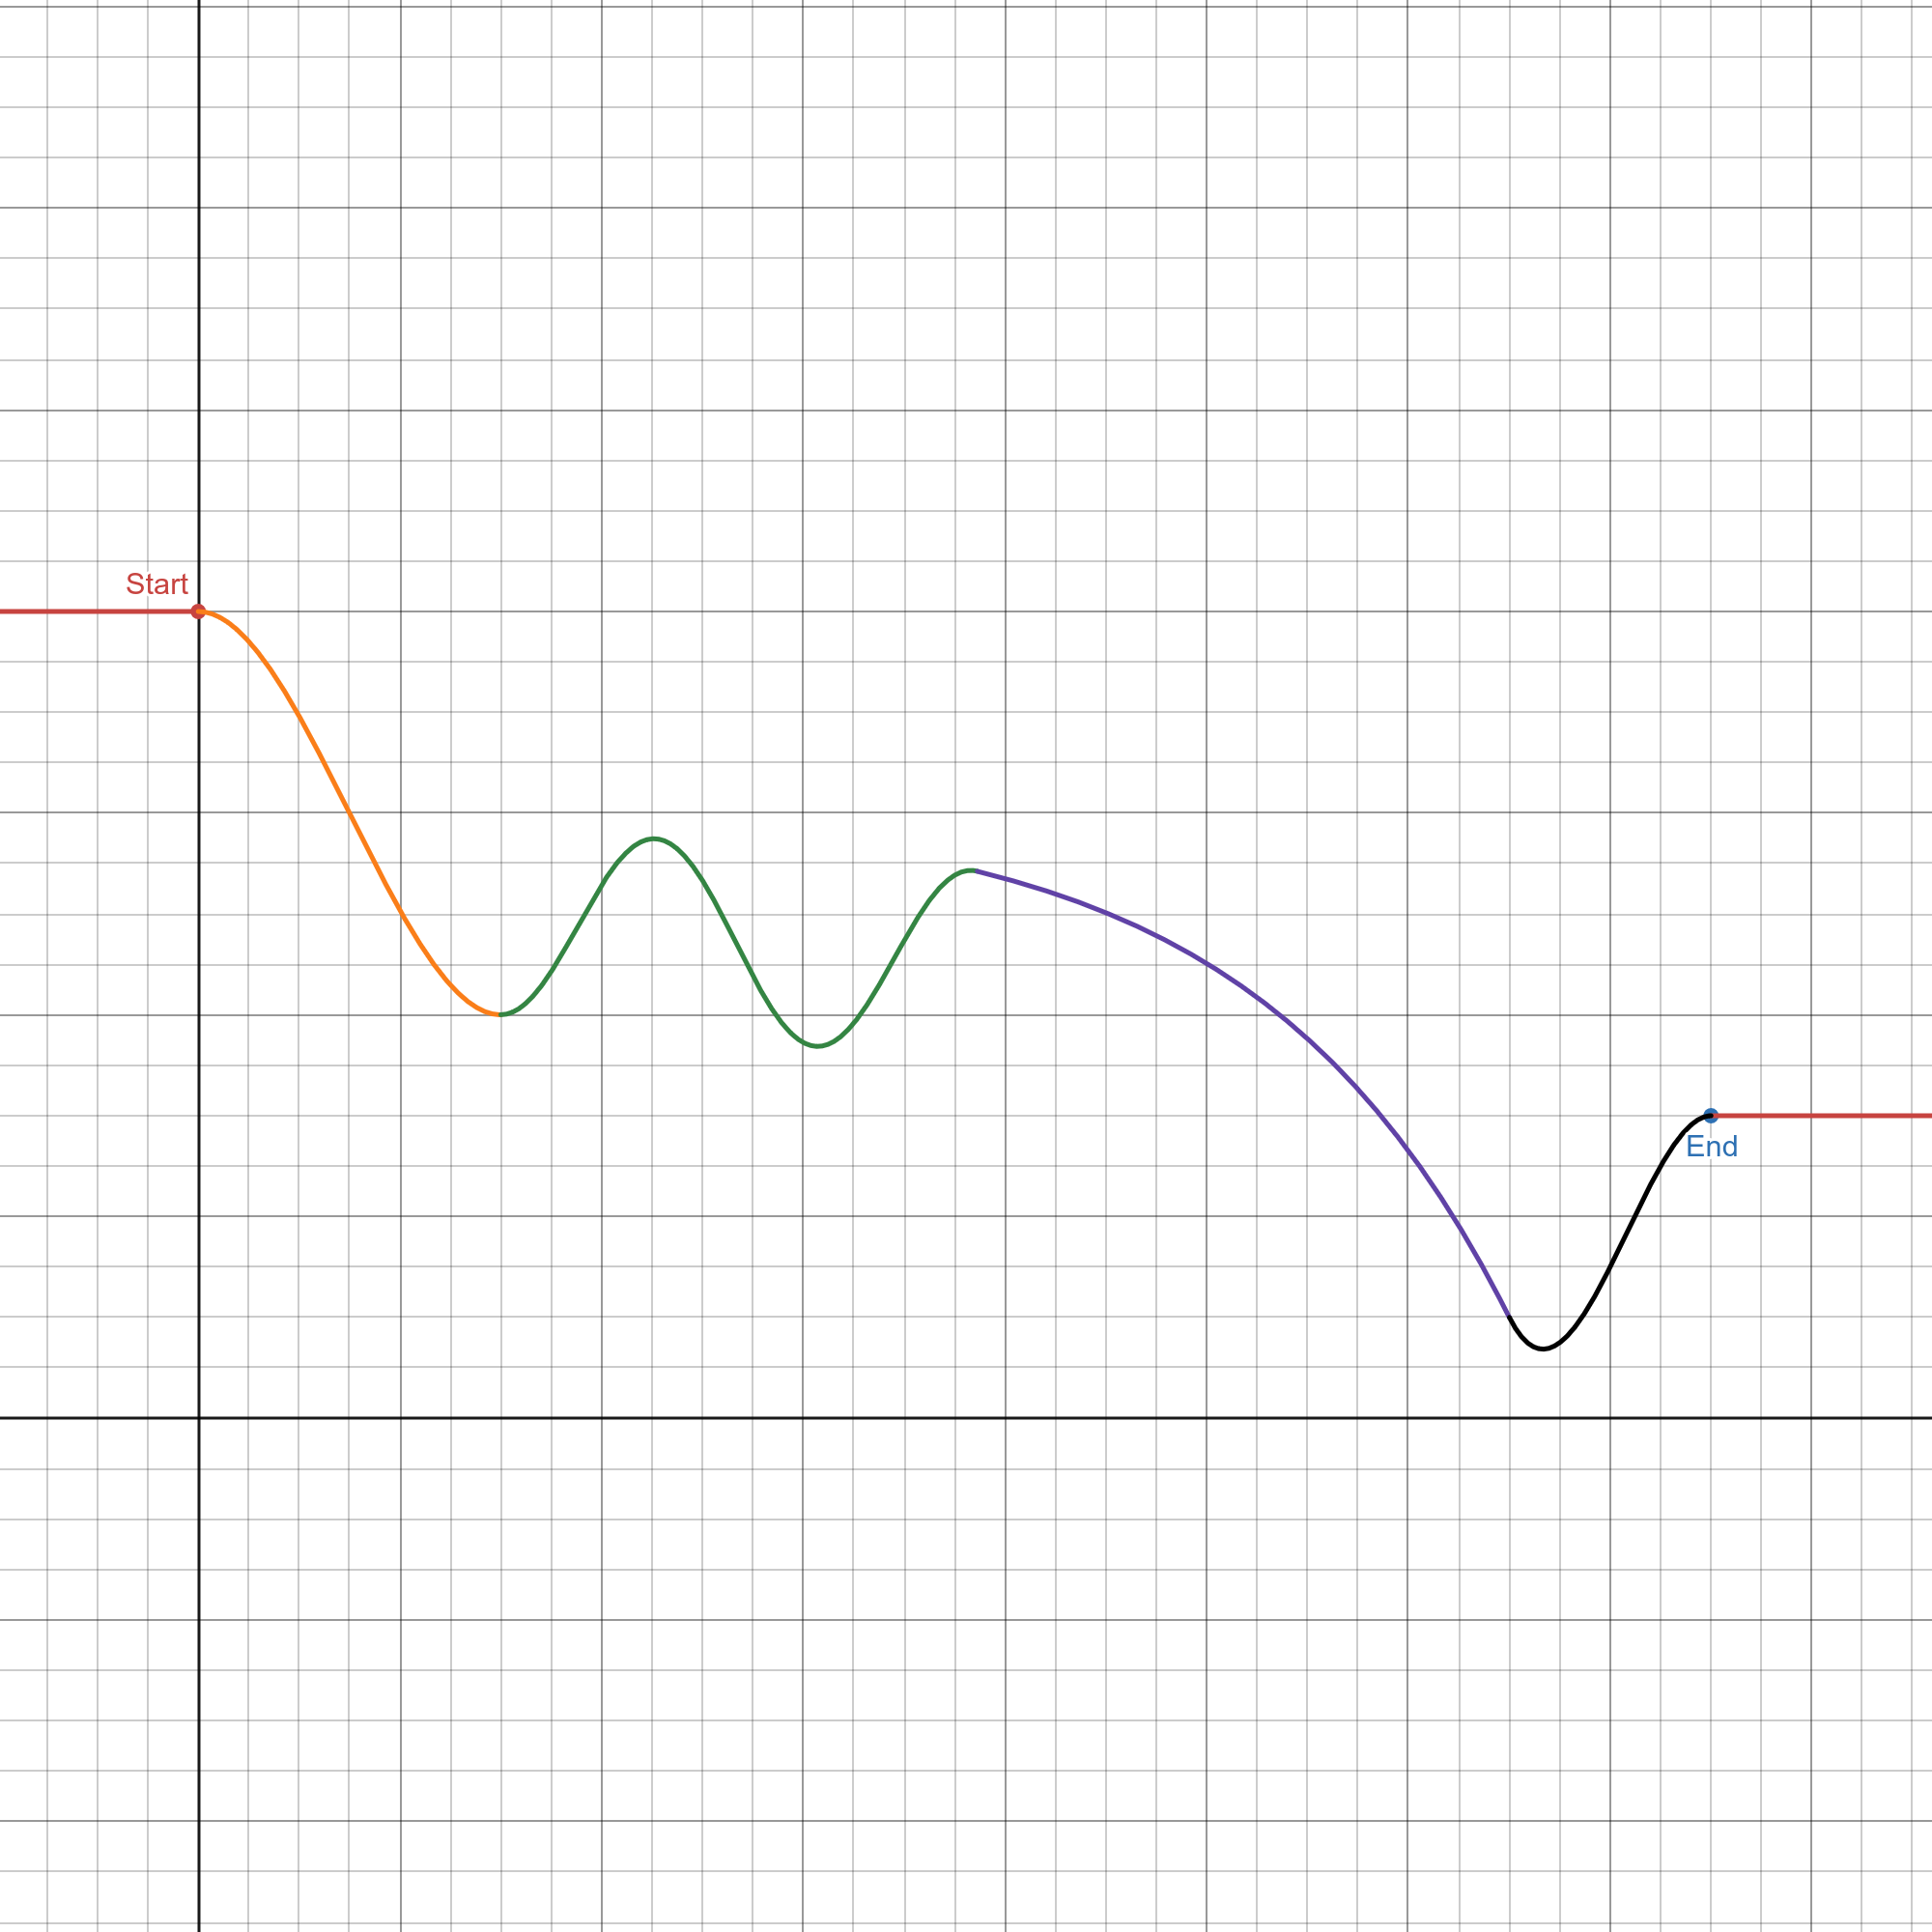
\includegraphics[width=1\linewidth]{finalgraph.png}
\begin{center}
	\large
	\vfill
	Maths Methods IA1
\end{center}
	
\end{titlepage}


\newpage
\tableofcontents


\newpage


\section{Formulation}
\subsection{Context}
Roller coasters are investment opportunities in which profit is largely affected by the amount of exhilaration they produce. While enticing passengers, and making a profit, are important factors, safety must also be considered. 
In this project, a roller coaster and support structure were designed using mathematical functions to cultivate maximum exhilaration and satisfactory safety, all while minimising costs.
\subsection{Assumptions and Observations}
The following assumptions and observations were made before, and throughout the completion of the task. The assumptions made are required prerequisites, or simplifications, that ensure a valid solution can be achieved.
The roller coaster was modelled in 2D to simplify calculations, and because graphing functions in 3D was out of the scope of the project. 
\begin{itemize}
	\item The task sheet specified "The beginning and end sections... have been erected and are in a perfectly straight alignment". While this did clarify that the first, and end pieces of track were parallel, their slope was not specified, and therefore assumed to be 0.
	
	\item The terminology "smooth" was used to describe the required transition between pieces of track. It is assumed that this implied that at transitions segments would be at same position and have the same gradient.
	
	\item The success criteria is maximum exhilaration, caused by "swift changes in direction, height and steepness". This could be could be translated to swift changes in the $y-$axis, and gradient. However if this was interpreted at face value, the ideal roller coaster would be a sine, or cosine function, with the lowest period possible. While this would fulfil the success criteria, it would not be enjoyable for passengers, and therefore caused them to be less exhilarated. Therefore while exhilarating features were incorporated, variation and comfort were considered as equally important. 
	
	\item For this task, the supporting structure under the track was required to consist of equally spaced main columns priced at \$180/metre, and interconnecting bracing priced at \$20/metre$^2$. It was assumed that placing support liberally to ensure sufficient integrity would be more cost effective than repairing catastrophic failure in the aftermath of improper placement.
	
	
	\item It was required that the track be constructed of at least 3 or more types of functions, including at least two types that are covered in Unit 3 Topic 2. The functions covered were exponential, logarithmic, and trigonometric functions.
	
	\item Trigonometric functions were calculated in radians, rather than degrees, in order for them to oscillate more with smaller change in $x$.
	
	\item In order for the roller coaster to have sufficient speed to overcome any peaks or hills in the track, each successive peak should be at a lower height than any preceding it.
	
\end{itemize}



\subsection{Translation of aspects to Mathematical concepts and techniques}

Since the roller coaster had been assumed to be 2D, it's track was represented on the Cartesian plane. This allowed the use of desmos to graph its track and perform calculations by letting 1 unit be 1 meter. 

Considering the track criteria provided, the start of the track should be at $(0, 80)$, and the end at $(150, 30)$.

\begin{figure}[h]
	\centering
	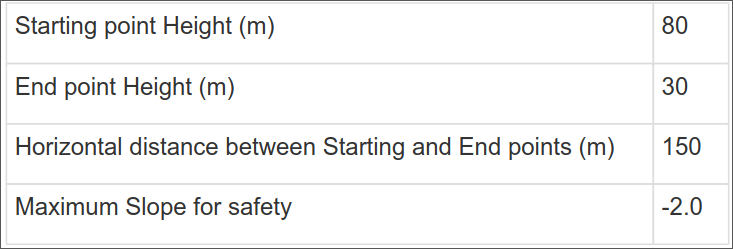
\includegraphics[width=10cm, trim=4 4 2 2,clip]{trackdefined.png}
	\caption{Track criteria}
\end{figure}
		\begin{figure}[h]
	
	\begin{center}
		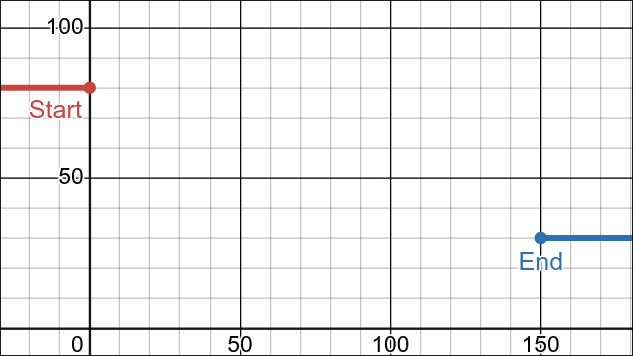
\includegraphics[width=10cm]{Start and End.png}
		
		\caption{Start and 
			End sections of the track}
	\end{center}
	
	
\end{figure}

The derivative function of modelled sections of track could be used to determine if the track exceeded the "maximum slope for safety" requirement provided by the task sheet.


In order to achieve as much of a thrill as possible, the maximum allowed slope should be reached whenever feasible while still incorporating change in gradient.
While the maximum slope is defined as $-2$, interpreting it directly as $-2\geq \textbf{slope}$ would result in a dangerously steep coaster that could only travel downwards. Henceforth any mention of a "maximum" or "highest possible" slope should be interpreted as "steepest negative", so that $-2\leq \textbf{slope}$.




\section{Solve}
\subsection{Modelling in Desmos}
\subsubsection{The First Function}

Considering that the starting point $(0, 80)$, there was already sufficient height for the maximum gradient to be reached for a reasonable duration.
The cubic function was found suitable as it forms 2 stationary points, useful for "smoothly" joining tracks.
Clearly the first function will intersect, and requires a gradient of $0$, at $(80, 0)$. Therefore initial requirements for the first function were:
$$f(x)=ax^3 +bx^2 +cx +d$$
$$f(0)=80\because\textrm{Vertical alignment}$$
$$f'(x)=0 \because \textrm{Smooth transition from beginning}$$
$$f'(0)=0\Rightarrow c=0\because \textrm{Variables with } x \textrm{ coefficient's become 0}$$

Since the derivative function was a quadratic, when $a>0$, its lowest point could be considered the maximum slope reached by the original.
The $x$-coordinate of the turning point could found using the vertex formula, which stated that for turning point $(x, y),\; x=\frac{-b'}{2a'}$. In this case, since there are other coefficients of $x^2$ and $x$ than $a$ and $b$ respectively, we let $a'=3a$, and $b'=2b$ when solving.

Considering the derivative function
 $$f'(x)=3ax^2+2bx$$
 $x$-coordinate of the turning point was: 
 $$\frac{-b'}{2a'}=\frac{-2b}{2\cdot3a}=\frac{-b}{3a}$$



\begin{figure}[h!]
	\centering
	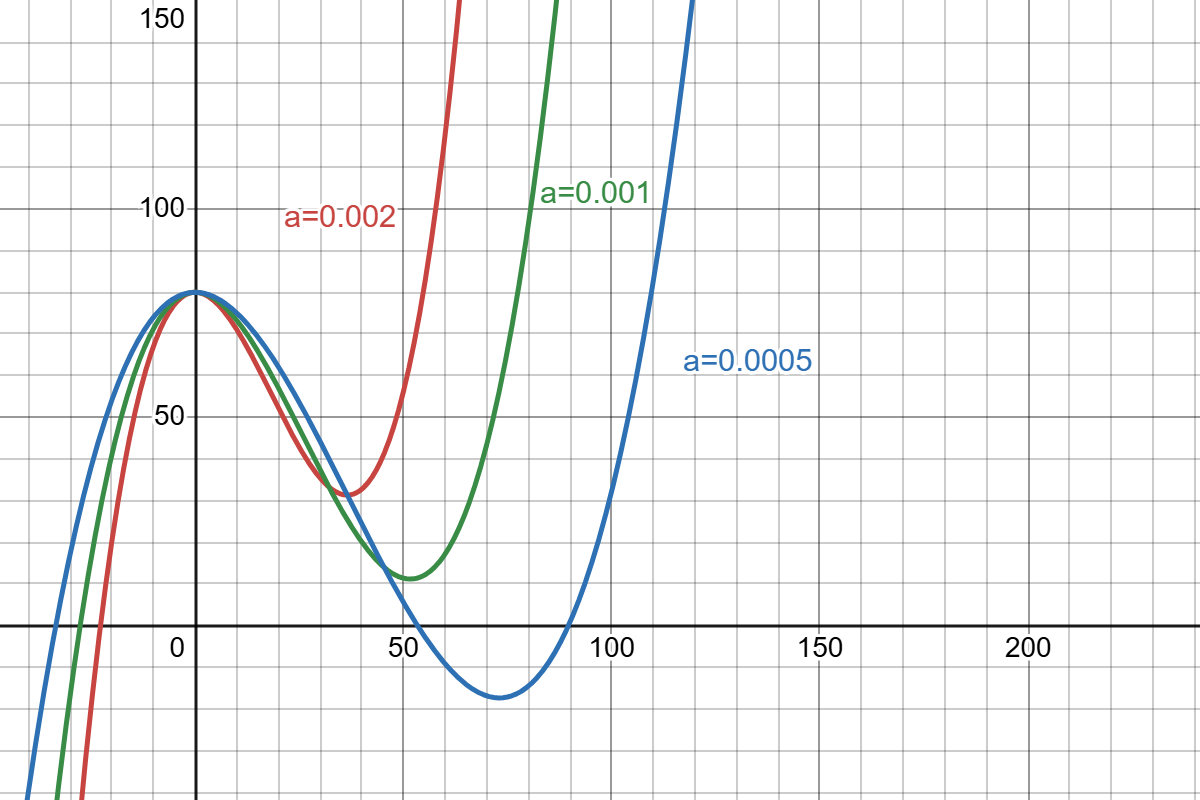
\includegraphics[width=10cm]{Eaxmple Cubic.png}
	\caption{$f(x)=ax^{3}-\sqrt{6a}x^{2}+80$ with various $\mathbf{a}$ values}
\end{figure}


Therefore by finding $f'(\frac{-b}{3a})=-2$, a generic function could be found with minimum gradient -2, located at turning point.
 $$f'(\frac{-b}{3a})=-2\Rightarrow b=\pm\sqrt{6a}$$
$$\therefore f(x)=ax^3\pm\sqrt{6a}x+d, a\geq0$$

$f(x)=ax^3-\sqrt{6a}x+80, a\geq0$ was inserted as it placed the "drop", and turning point on the right side of the start of the coaster.

The end of the first function was chosen to be $f(30)$ to maintain sufficient altitude.

To make joining the next function easier, $f'(30)=0$ was considered. 

$$f'(30)=0 \Rightarrow a=\frac{2}{675}$$

$$\therefore f(x)=\frac{2}{675}x^{3}-\frac{2}{15}x^{2}+80$$


\subsubsection{The Second Function}
The sine function was ideal for "swift changes in direction, height, and steepness", and possessed infinite stationary points. It was chosen to be the second function.

Considering 
$$s(x)=a\sin(b(x+c))+d $$
$$s'(x)=ab\cos(b(x+c))$$

Clearly the maximum downwards gradient was defined by $$ab\cdot-1$$
when
$$\cos(b(x+c))=-1$$

However the peak of the next oscillation was the same height than the previous one. Therefore new function was created to ensure passengers had sufficient speed to overcome the next peak.

Considering
$$c(x)=a\sin(b(x+c))+d+gx$$ 
$$c'(x)=ab\cos(b(x+c))+g$$

Clearly now when $g<0$, the function will slope downwards throughout its oscillation. 

	\begin{figure}[h!]
		\centering
		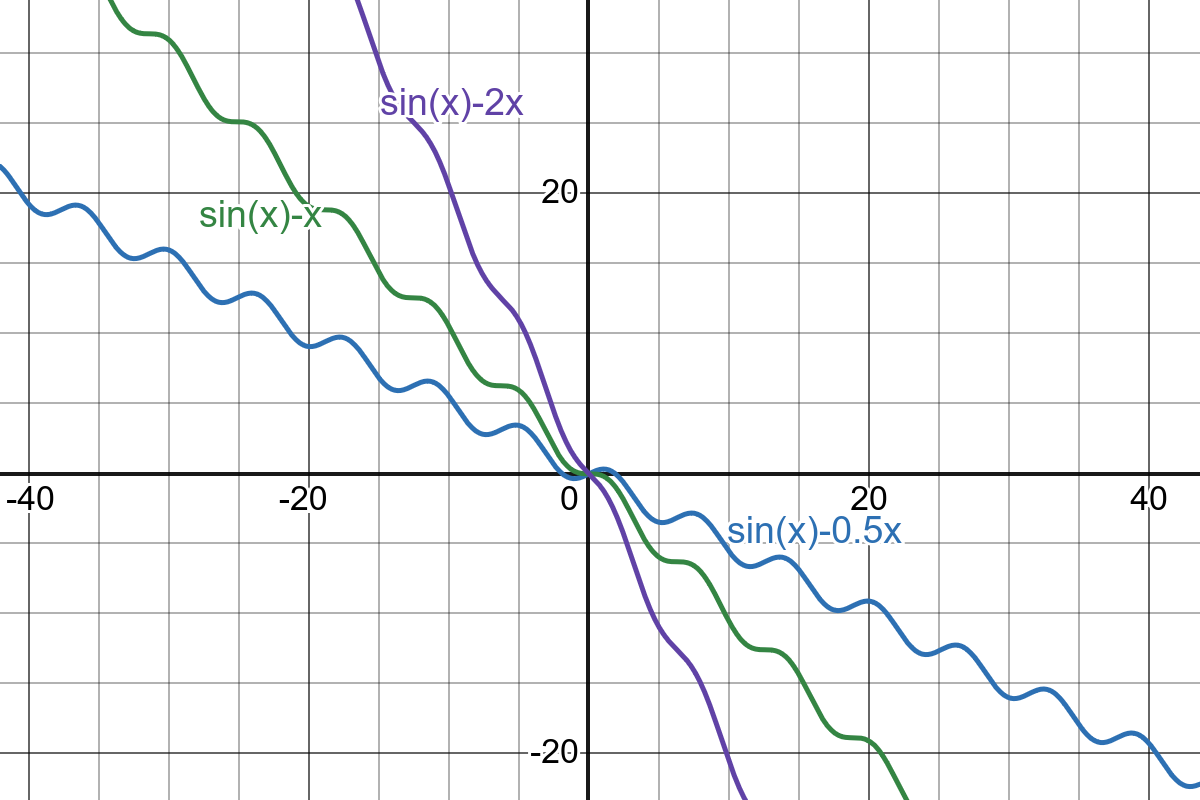
\includegraphics[width=10cm]{c(x).png}
		\caption{$y=sin(x)$ with various slopes applied}
	\end{figure}



When $g=-0.1$, clearly $ab\cdot -1-0.1=-2$ would result in a minimum gradient of $-2$. Through trial and error in desmos it was found that $c'(x)=-2$, $a=9.5$ and $b=0.2$ were appropriate. To align the functions, $f'(x)=c'(x)$ was considered. The function was shifted horizontally by letting $c'(30)=f'(30)$, and choosing an appropriate solution for $c$ where the minimums were aligned. The function was then shifted vertically, by letting $c(30)=f(30)$, altering $d$ until the functions met.  

It was found  that

 $$f'(30)=9.5\cdot0.2\cos (0.2(30+c))-0.1=0 \Rightarrow c=-6.174775557$$

$$\therefore f(30)=9.5\sin(0.2(30-6.174775557))+d+3=40 \Rightarrow d=52.48683298$$

\subsubsection{The Third Function}
It was decided that the third function would be an exponential with decreasing gradient and height to utilise the remaining altitude and increase speed.

Considering the general form of an exponential, $g(x)=ae^{b(x+c)}+d$, it was found that solving for variables $a, b, c$ and $d$ would require significant computation.

Therefore it was decided that by letting $c=0$, and $d=0$, only $a$ and $b$ would need to be solved for. 

Due to elimination of horizontal or vertical shifting, the point $(80, 0)$ was considered the origin for $g(x)$, so that  initial requirements such as $g(80)=c(80)$ became $g(0)=c(80)$. 

It was required that 
$$g'(0)=c'(80) \because \textrm{Smooth transition}$$
$$g(0)=c(80)\because \textrm{Alignment}$$ 
$$g'(50)=-2\because \textrm{Desired final gradient}$$

Solving with simultaneous equations gave 
$$a=\frac{c'(80)}{be^{80b}}$$ 

$$\therefore g(80)=\frac{c'(80)}{be^{80b}}\cdot e^{80b}\Rightarrow b=\frac{c'(80)}{c(80)}\approx -0.023308398873$$

However this solution intersected with the $x-\textrm{axis}$ prematurely. 
	\begin{figure}[h]
		\centering
		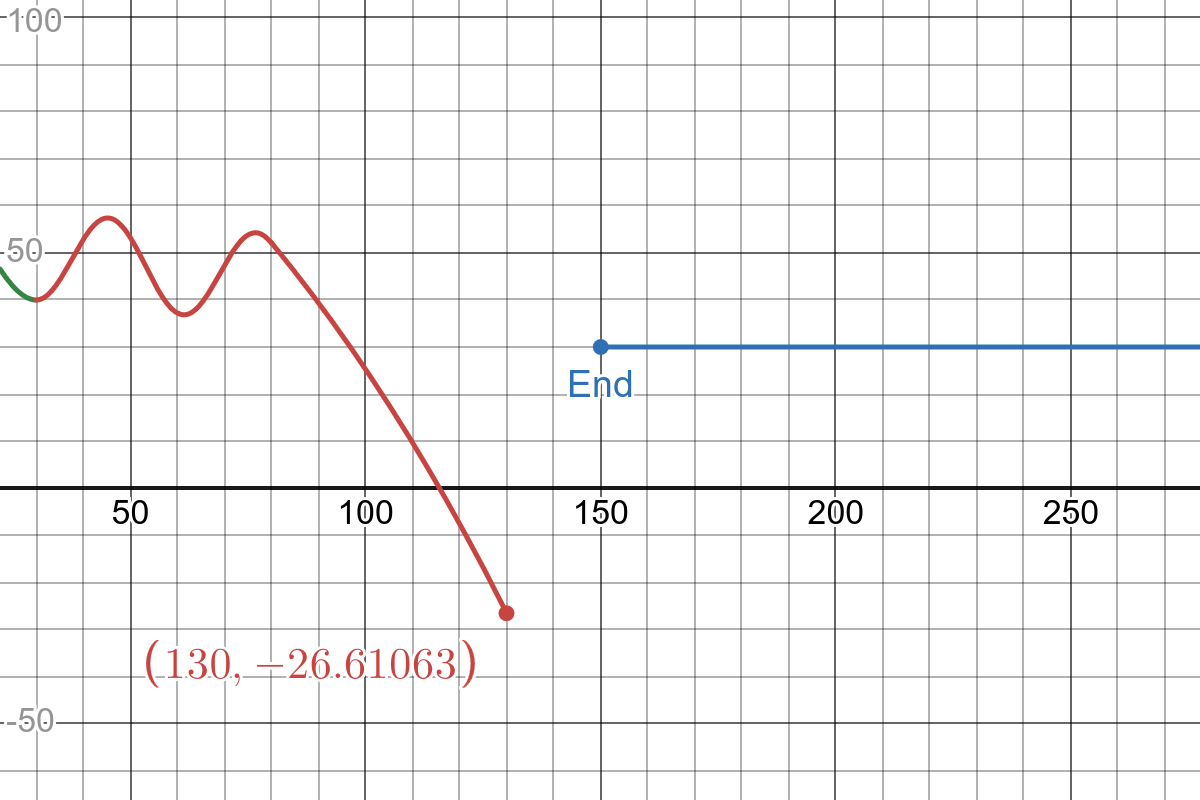
\includegraphics[width=10cm]{PrematureIntersecion.png}
		\caption{$g(x)$ intersecting with the $x-\textrm{axis}$}
	\end{figure}


	

By considering $s'(\lambda)=g'(0)$, a suitable $x$ value for the starting point of the function was defined, which did not cause contradictions when later conditions were established. 

This was rearranged to give $$a=\frac{s'(\lambda)}{b}$$

Substituting into $g'(\gamma)=-2$
 
 $$g'(\gamma)=-2=s'(\lambda)e^{\gamma b}\Rightarrow 
 b=\frac{1}{\gamma}\ln(\frac{-2}{s'(\lambda)})$$ Substituting into $g(x)=ae^{bx}$

 $$g(x)=\frac{s'(\lambda)}{\frac{1}{\gamma}\ln(\frac{-2}{s'(\lambda)})}\cdot e^{\frac{1}{\gamma}\cdot \ln (\frac{-2}{s'(\lambda)})\cdot x}$$ 
 
 Now for $g(x)$:
 \begin{itemize}
 	\item $\gamma$ is the distance that the function takes to reach $g'(x)=-2$
 	\item $\lambda$ is the $x$ value that the joins with the previous function, $s(x)$.
 \end{itemize}
		

Instanced of $x$ were replaced with $(x-\lambda)$ horizontally shift, and "$+s(\lambda)-a$" was inserted at the end to vertically shift so that $g(\lambda)=s(\lambda)$.
		

It was required that the equation terminate at $g(x)=10$ so that there would be room for the final function to invert direction and climb. Therefore $g(\lambda + \gamma)=10$, where $\gamma=130-\lambda$, was considered, as this would ensure that $g'(\lambda-\lambda-130)=g'(130)=-2$, while still allowing for $\lambda$ to be altered until a suitable answer was found.
		

It was found that for 
$$g'(130)=-2 \textrm{ and } g(130)=10$$ 

$$\lambda=77.2487110854776$$ 

$$\therefore g(x)=\frac{s'(\lambda)}{\frac{1}{\gamma}\ln(\frac{-2}{s'(\lambda)})}\cdot e^{\frac{1}{\gamma}\cdot \ln (\frac{-2}{s'(\lambda)})\cdot (x-\lambda)}+s\left(\lambda\right)-\frac{s'(\lambda)}{\frac{1}{\gamma}}\ln\left(\frac{-2}{s'\left(\lambda\right)}\right)$$ where $$\lambda=77.2487110854776$$
$$\gamma=130-\lambda$$





\subsubsection{The Fourth Function}

The final function was decided to be a cubic function, as multiple turning points were required, and the process for defining a cubic with constraints had already been established when creating the first function. 
	

Requirements for cubic $f_2(x)=a_2x^3+b_2x^2+c_2x+d_2$ were:

$$f_2'(130)=g'(130)$$
$$f_2(130)=g(130)$$
$$f_2'(150)=0$$
$$f_2(150)=30$$
	
However to simplify calculations, alternative requirements were considered.
$$f_2'(0)=g'(130)\because \textrm{Smooth transition}$$
$$f_2(0)=g(130)\because \textrm{Alignment}$$
$$f_2'(20)=0\because\textrm{Smooth transition}$$
$$f_2(20)=30\because\textrm{Alignment with end} $$

Horizontal shift was later accounted for by substituting instances of $x$ with $(x-130)$
	

Solving simultaneously for these conditions gave values 
	
	$$a_{2}=\frac{g'\left(130\right)+40b_{2}}{-1200}$$
	
	$$b_{2}=\frac{3}{400}\cdot\left(30-\frac{g'\left(130\right)\cdot8000}{-1200}-\left(20\cdot g'\left(130\right)\right)-g\left(130\right)\right)$$
	
	$$c_{2}=g'\left(130\right)$$
	
	$$d_{2}=g\left(130\right)$$

For further working see appendix $\mathbf{A}$
	


\subsection{Final Functions
}

$$
\begin{Bmatrix}
	\frac{2}{675}x^{3}-\frac{2}{15}x^{2}+80 & 0\le x<30 \\
	9.5\sin(0.2(x-6.174775557))-0.1x+52.48683298  & 30\le x<77.2487110854776 \\
	-6.24204780148\cdot e^{0.0396232574628(x-77.2487110854776)} + 60.4754058113 & 77.2487110854776 \leq x < 130 \\
	
	-0.01(x-130)^{3}+0.35\left(x-130\right)^{2}+-2\left(x-130\right)+10 & 130\le x\leq150
	
\end{Bmatrix}
$$




\subsection{Supporting Structures}
columns were defined by:

$$x=k_{4}\left\{0\le y\le f\left(x\right)\right\}$$

$$x=k_{4}\left\{0\le y\le c\left(x\right)\right\}$$

$$x=k_{4}\left\{0\le y\le g\left(x\right)\right\}$$

$$x=k_{4}\left\{0\le y\le f_{2}\left(x\right)\right\}$$

where

$$k_{1}=\left[1,2,3,5,6,10,15,25,30,50,75,150\right]$$

$$k_{2}=\left[0...\frac{150}{k_{1}\left[k_{3}\right]}\right]$$

$$k_{3}=4$$

$$k_{4}=k_{1}\left[k_{3}\right]\cdot k_{2}$$

This ensures that there will always be support at the start and end of the track, while allowing the density of supports to be easily altered via $k_3$ when $1\leq k_3\leq12$

Summating the result of each function at the $x$ value of each column gave the total length of column required in meters. Multiplying this by the cost per meter gave the total cost for columns.



$$t_{1}=\sum_{n=0}^{6}\left(f\left(n\cdot5\right)\right)$$
$$t_{2}=\sum_{n=7}^{15}c\left(5n\right)$$
$$t_{3}=\sum_{n=16}^{25}g\left(5n\right)$$
$$t_{4}=\sum_{n=26}^{30}f_{2}\left(5n\right)$$
$$t_{total}=\left(t_{1}+t_{2}+t_{3}+t_{4}\right)\cdot180$$

Summating the definite integral of each function that is track is constructed by over their domain gives the total area that requires interconnecting bracing. Multiplying this by the cost per meter$^2$ gave the total cost for bracing.

$$i_{1}=\int_{0}^{30}f\left(x\right)dx$$
$$i_{2}=\int_{30}^{\lambda}c\left(x\right)dx$$
$$i_{3}=\int_{\lambda}^{130}g\left(x\right)dx$$
$$i_{4}=\int_{130}^{150}f_{2}\left(x\right)dx$$
$$i_{total}=\left(i_{1}+i_{2}+i_{3}+i_{4}\right)\cdot20$$


 $$\therefore \textrm{Cost}_{\mathrm{total}}=t_\mathrm{total}+i_\mathrm{total}=241739.758457+128797.817705=370537.576162$$

Therefore the total cost of the roller coaster was $\$370,537.58$
\section{Evaluate and Verify}
\subsubsection{Reasonableness}



The assumption that the start and end pieces had a slope of 0 was found to be optimal for joining them to the turning points of the inside functions. However, if it was instead assumed that the start and end pieces of track were slanted, with a gradient of, say $-2$, then the roller coaster would be more thrilling, as the passengers would be travelling faster and experience greater forces.


While simplification of the model to 2D did make the roller coaster less thrilling, as passengers would only experience thrilling movements in 2 dimensions, rather than 3, it greatly simplified calculations as intended


\subsubsection{Strengths}
While the actual level of exhilaration cannot be measured, as the model is purely theoretical, the solution has been deemed successful due to the successful incorporation of exhilarating features, and the consideration comfort and variation across such features.

The function $c(x)$ had the largest changes in gradient, which theoretically contributed the largest thrill to passengers. Additionally, it not only reached the maximum slope throughout its oscillation, but ensured that passengers maintained enough speed to overcome each one of its peaks through its integrated linear function.

While the cubic function was utilised heavily, the requirements for there to be at least two types of functions that were covered in Unit 3 Topic 2 included in the roller coaster and least 3 types of functions overall, were fulfilled.



\subsubsection{Limitations}


The organisation and labelling of functions and variables throughout the solution was inconsistent and confusing. Variables, such as $b$, were often defined multiple times in different functions. A better naming scheme was adopted toward the end of the task, with the last function becoming $f_2(x)$, rather than an arbitrary letter. 

Many variables lacked exact solutions. This resulted functions which lacked readability and accuracy, however, the rounding errors were assumed inconsequential, and were imperceivable against exact solutions, considering the real world scale.

Cost of the attraction was considered when placing the supports after the design had been finalised, rather than during the design or refinement process. Lowering the coaster would result in lower support costs, but less of a thrill from the final drop along $g(x)$. 

Being restricted to equally spaced main columns means that rather than placing fewer, but more intentionally placed, columns meant that the amount of columns had to be increased in order to support sections of the track misaligned, or under higher load. Additionally, rather than calculating the load on the track, column spacing was decided arbitrarily.
\section{Conclusion}
In this project, an exhilarating roller coaster was modelled and defined by the functions $f(x), c(x), p(x),$ and $f_2(x)$, which were found through substituting and simultaneously solving for specific values, the values of each other, the value of their derivative, or the value of each others derivatives. While much of the process involved imprecise measurement and arbitrary decisions, the final result was considered to be varied, and exhilarating. 

The total cost was $\$370,537.58$. While we lack a frame of reference to evaluate the reasonableness of the cost against, cost reducing measures would have decreased the exhilaration the coaster caused, therefore it was decided that the current cost-to-exhilaration ratio was satisfactory.



\begin{appendices}

	\section{The Fourth Function}
	$f_2(0)=g(130)\Rightarrow d=g(130)$
	
	$f_2'(0) = g'(130)\Rightarrow c=g'(130)$
	
	$f'(20)=0\Rightarrow a=1200a+40b+g'(130)$
	
	
\end{appendices}





\end{document}